%%============
%%  ** Author: Shepherd Qirong
%%  ** Date: 2021-12-11 17:07:45
%%  ** Github: https://github.com/ShepherdQR
%%  ** LastEditors: Shepherd Qirong
%%  ** LastEditTime: 2021-12-12 14:28:48
%%  ** Copyright (c) 2019--20xx Shepherd Qirong. All rights reserved.
%%============



\documentclass[UTF8]{article}
\usepackage{ctex}
\usepackage{amsmath,amsthm,amsfonts,amssymb,bm,mathrsfs,upgreek} 
\usepackage{graphicx}
\usepackage[paper=a4paper,top=3.5cm,bottom=2.5cm,
left=2.7cm,right=2.7cm,
headheight=1.0cm,footskip=0.7cm]{geometry}
\usepackage{color}
\usepackage{multirow,booktabs}

\RequirePackage{setspace}%%linespace
\setstretch{1.523}


\begin{document}
\section{Introduction}
Today is 20211211, and I deciede to note down all of my knowledge about problems in this notebook. Actually we think for a while whether to seperatre the knowledge into different documents.

\section{Physics}

\subsection{Energy}

\subsubsection{T0001}
The coordinate of free fall ball ends. With energy equation, we have $GH = \mu G \xi kH$, considering of the backward length, we draw the figure and it can be transfered from the figure $y = |x|$. We have the coordinate
at $[1-\vert (\mu k)^{-1} \pmod 2 -1 \vert ]kH $.
\begin{figure*}[h]
    \centering
    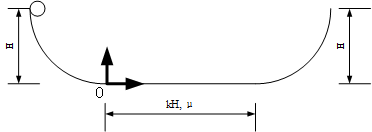
\includegraphics[width=0.5\textwidth]{../../resources/T0001.png}
    \caption{[T0001: Where the ball ends]}
    \label{fig:1}
\end{figure*}

\subsubsection{T0002}
Suppose the ball free falls tangently into a circle, at the top of the circle, to matian the circular movement, $mg + F_{support} = mv^2/R$, since $m(n-2)gR = 1/2mv^2$, we have $F_{support} = mg(2n-5)$.

When $n<=1$, it is easy to see that the ball swings. When $n>=2.5$, the ball keeps going along the circle. When $n \in (1,2.5)$, suppose the ball is at the angle $\theta$ as shown in the figure, the energy equation shows that $(nR-R + R \cos \theta) mg = 1/2 mv^2$, force equation shows that $F_{support} - mg \cos \theta = m v^2/R = 2mg(n-1+\cos \theta )$, so $F_{support}  = mg(2n-2+ 3\cos \theta )$. when $F_{support}  = 0$, the ball falls, and it falls at the angle $ \cos \theta = \frac{2}{3}(1-n)$.
\begin{figure*}[h]
    \centering
    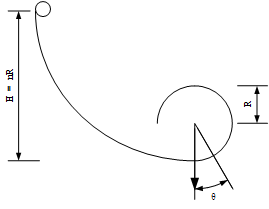
\includegraphics[width=0.5\textwidth]{../../resources/T0002.png}
    \caption{[T0002: Where the ball falls]}
    \label{fig:2}
\end{figure*}

\subsubsection{T0003}
When an object seperates into several parts, the velocity of each component is different. Using the momentum equation, we have $mv = (-dm)u+(v+dv)(m+dm)$, and we let $u = v+dv-v_{rel}$, so we have $0 = v_{rel} dm + m dv$, so $dv = -v{rel} \frac{dm}{m}$, the formula is integrated as $v_{final} - v_{0} = v_{rel} \ln \frac{m_0}{m_{final}}$. This means that when the rocket accolerates like this, the final mass needs to be quite small, because the logarithm function decreases rapidly, also the $v_{rel}$ needs to be big.

\begin{figure*}[h]
    \centering
    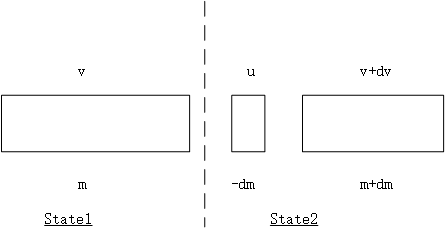
\includegraphics[width=0.5\textwidth]{../../resources/T0003.png}
    \caption{[T0003: Where the ball falls]}
    \label{fig:3}
\end{figure*}


\end{document}